\documentclass[12pt]{article}
\usepackage[a4paper, margin=1in]{geometry}
\usepackage[document]{ragged2e}
\usepackage{graphicx}
\graphicspath{ {./images/} }
\usepackage{enumerate}
\usepackage{framed}
\usepackage{amsmath,amsfonts,amsthm,thmtools,amssymb,mathtools,commath}
\usepackage{physics}
\usepackage{tikz}
\usetikzlibrary{mindmap}
\usepackage{caption}
\usepackage{xcolor}
\usepackage[most]{tcolorbox}
\usepackage{cleveref}


%%%%%%%%%%%%%%%%
%  Definition  %
%%%%%%%%%%%%%%%%
\tcbuselibrary{theorems,skins,hooks}
\newtcbtheorem[number within=subsection]{definition}{Definition}%
{
    % theorem style=definition,
    enhanced,
	before skip=2mm,after skip=2mm, colback=cyan!5,colframe=cyan!80!black,boxrule=0.5mm,
	attach boxed title to top left={xshift=1cm,yshift*=1mm-\tcboxedtitleheight},
	boxed title style={frame code={
					\path[fill=cyan]
					([yshift=-1mm,xshift=-1mm]frame.north west)
					arc[start angle=0,end angle=180,radius=1mm]
					([yshift=-1mm,xshift=1mm]frame.north east)
					arc[start angle=180,end angle=0,radius=1mm];
					\path[left color=cyan!30!black,right color=cyan!30!black,
						middle color=cyan!50!black]
					([xshift=-2mm]frame.north west) -- ([xshift=2mm]frame.north east)
					[rounded corners=1mm]-- ([xshift=1mm,yshift=-1mm]frame.north east)
					-- (frame.south east) -- (frame.south west)
					-- ([xshift=-1mm,yshift=-1mm]frame.north west)
					[sharp corners]-- cycle;
				},interior engine=empty,
		},
	fonttitle=\bfseries,
	title={#2},#1
}{def}


%%%%%%%%%%%%%
%  Theorem  %
%%%%%%%%%%%%%
\tcbuselibrary{theorems,skins,hooks}
\newtcbtheorem[use counter from=definition]{theorem}{Theorem}%
{
    theorem style=plain,
    enhanced,
    colframe=green,
    boxrule=1pt,
    titlerule=0mm,
    toptitle=1mm,
    bottomtitle=1mm,
    fonttitle=\bfseries,
    fontupper=\mdseries\itshape,
    coltitle=green!30!black,
    colbacktitle=cyan!15!white,
    colback=green!10,
    description font=\bfseries\sffamily
}{thrm}


%%%%%%%%%%%%%%
% Corollary  %
%%%%%%%%%%%%%%
 \tcbuselibrary{theorems,skins}
 \newtcbtheorem[use counter from=theorem]{corollary}{Corollary}%
 {
    theorem style=plain,
    enhanced,
    colframe=green,
    frame hidden,
    titlerule=0mm,
    toptitle=1mm,
    bottomtitle=1mm,
    fonttitle=\bfseries,
    fontupper=\mdseries\itshape,
    coltitle=green!30!black,
    colbacktitle=cyan!15!white,
    colback=green!10,
    description font=\bfseries\sffamily
 }{corl}


%%%%%%%%%%%%%
%  Example  %
%%%%%%%%%%%%%
\tcbuselibrary{theorems,skins,hooks}
\newtcbtheorem[number within=section]{example}{Example}%
{
	enhanced,
	breakable,
	colback = gray!5,
	frame hidden,
	boxrule = 0sp,
	borderline west = {2pt}{0pt}{gray},
	sharp corners,
	detach title,
	before upper = \tcbtitle\par\smallskip,
    coltitle=gray!70!black,
	fonttitle = \bfseries\sffamily,
	description font = \mdseries\bfseries
}
{xmp}


%%%%%%%%%%%%%%
%  Exercise  %
%%%%%%%%%%%%%%
\tcbuselibrary{theorems,skins,hooks}
\newtcbtheorem[number within=section]{exercise}{Exercise}%
{
    enhanced,
    breakable,
    colback=black!5,
    colframe=black!30,
    left=0.5em,
    before skip=10pt,
    after skip=10pt,
    boxrule=0pt,
    boxsep=0pt,
    arc=0pt,
    outer arc=0pt,
    borderline west={3pt}{0pt}{black!30},
}{exc}

%%%%%%%%%%
%  Note  %
%%%%%%%%%%
\usetikzlibrary{arrows,calc,shadows.blur}
\tcbuselibrary{skins}
\newtcolorbox{note}[1][]{%
	enhanced jigsaw,
	colback=gray!20!white,%
	colframe=gray!80!black,
	size=small,
	boxrule=1pt,
	title=\textbf{Note:-},
	halign title=flush center,
	coltitle=black,
	breakable,
	drop shadow=black!50!white,
	attach boxed title to top left={xshift=1cm,yshift=-\tcboxedtitleheight/2,yshifttext=-\tcboxedtitleheight/2},
	minipage boxed title=1.5cm,
	boxed title style={%
			colback=white,
			size=fbox,
			boxrule=1pt,
			boxsep=2pt,
			underlay={%
					\coordinate (dotA) at ($(interior.west) + (-0.5pt,0)$);
					\coordinate (dotB) at ($(interior.east) + (0.5pt,0)$);
					\begin{scope}
						\clip (interior.north west) rectangle ([xshift=3ex]interior.east);
						\filldraw [white, blur shadow={shadow opacity=60, shadow yshift=-.75ex}, rounded corners=2pt] (interior.north west) rectangle (interior.south east);
					\end{scope}
					\begin{scope}[gray!80!black]
						\fill (dotA) circle (2pt);
						\fill (dotB) circle (2pt);
					\end{scope}
				},
		},
	#1,
}

\usepackage{makecell}
\usepackage{subfigure}
\renewcommand{\thesubsection}{\arabic{subsection}}

\title{
    \textbf{EEE-184}\\
    \textbf{Experiment No. 1}
}

\author{
    Turja Roy\\
    ID: 2108052
}
\date{}

\begin{document}
\maketitle

\subsection{Write the name of different kinds of machines in the EML}
\subsubsection*{Answer:}
Different kinds of machines in the EML are:
\begin{enumerate}
    \item DC Generator
    \item DC Motor
    \item Transformer
    \item AC Motor
    \item AC Generator
    \item Induction Motor
    \item Synchronous Motor
    \item Break Motor
\end{enumerate}

\begin{figure}[h]
    \centering
    \subfigure{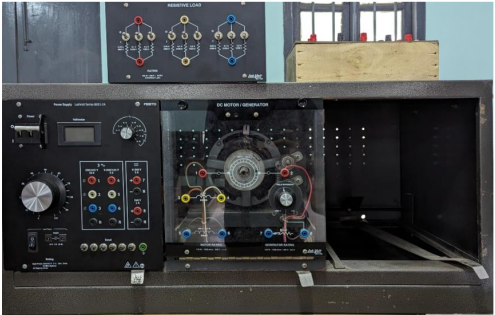
\includegraphics[width=0.4\textwidth]{./1.1.png}}
    \subfigure{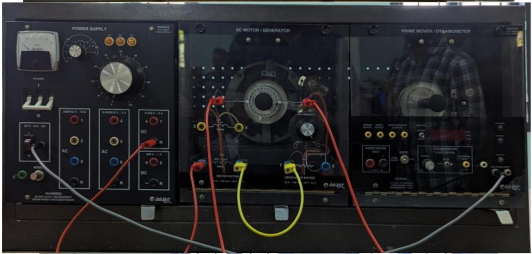
\includegraphics[width=0.5\textwidth]{./1.2.png}}
    \subfigure{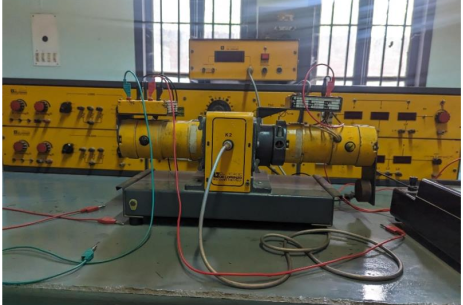
\includegraphics[width=0.4\textwidth]{./1.3.png}}
    \subfigure{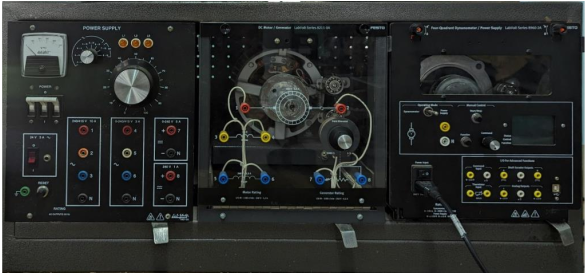
\includegraphics[width=0.5\textwidth]{./1.4.png}}
\end{figure}

\begin{figure}[h]
    \centering
    \subfigure{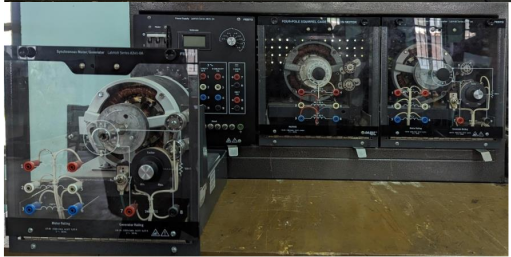
\includegraphics[width=0.4\textwidth]{./1.5.png}}
    \subfigure{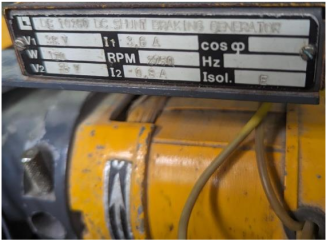
\includegraphics[width=0.4\textwidth]{./1.7.png}}
    \subfigure{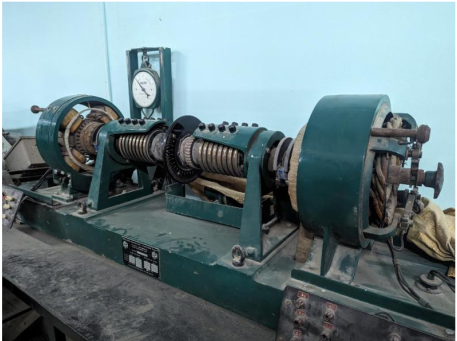
\includegraphics[width=0.4\textwidth]{./1.8.png}}
    \subfigure{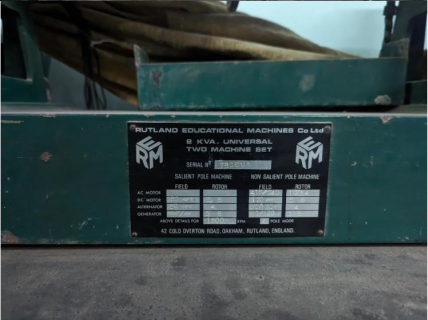
\includegraphics[width=0.4\textwidth]{./1.9.png}}
    \subfigure{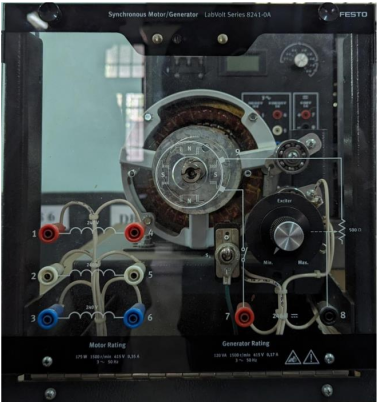
\includegraphics[width=0.4\textwidth]{./1.6.png}}
\end{figure}

\subsection*{}
\subsection{What are the types of power supply in the EML?}
\subsubsection*{Answer:}
There are two types of power supply in the EML:
\begin{enumerate}
    \item AC Power Supply
    \item DC Power Supply
\end{enumerate}

\subsection{Discuss about the different types of DC machines.}
\subsubsection*{Answer:}
Direct current (DC) machines are electromechanical devices that convert electrical energy into mechanical energy or vice versa through the interaction of magnetic fields. There are two main types of DC machines: DC generators (or dynamos) and DC motors. The components of DC machines are generally similar for both types, with some variations in their construction and. operation.

\begin{figure}[htpb]
    \centering
    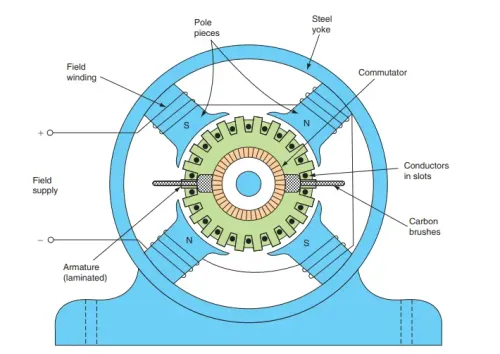
\includegraphics[width=0.5\textwidth]{./3.png}
\end{figure}

\begin{enumerate}
    \item \textbf{Stator (Field System): } The stator, or field system, is the stationary part of the DC machine that produces the magnetic field. It consists of the following components:
        \begin{itemize}
            \item \textbf{Field Windings: } Coils of wire wound around the pole pieces (field poles). These windings creatwe the magnetic field when current passes through them.\item \textbf{Field Poles: } Pieces of magnetic material attached to the frame or yoke of the machine. The field windings are wound around these poles.
        \end{itemize}
    \item \textbf{Rotor (Armature): } The rotor is the rotating part of the DC machine where the electromechanical energy conversion takes place. It comprises the following elements:
        \begin{itemize}
            \item \textbf{Armature Windings: } Conductors, usually in the form of coils, wound on the armature core. These windings carry the current that interacts with the magnetic field to produce torque or generate voltage:
            \item \textbf{Armature Core: } A stack of thin steel laminations, insulated from each other, that are mounted on the shaft. The armature windings are wound on the armature core.
            \item \textbf{Commutator: } A cylindrical arrangement of copper segments insulated from each other and from the shaft. The armature windings are connected to the commutator segments.
            \item \textbf{Brushes: } Carbon blocks or brushes that are held in contact with the commutator segments by brush holders. The brushes are connected to the external circuit through the brush holders.
        \end{itemize}
    \item \textbf{Shaft and Bearings: } The shaft supports the armature and allows it to rotate freely. Bearings provide support and reduce friction between the rotating armature and the stationary components.    
    \item \textbf{Yoke: } The yoke is the outer frame of the machine that supports the field poles and provides mechanical support for the machine.
    \item \textbf{Cooling System: } DC machines often have cooling systems to dissipate heat generated during operation. This could include fans, ventilation, or liquid cooling mechanism to maintain optimal operating temperatures.
    \item \textbf{Terminal Box or Terminals: } Terminals or a terminal box are provided for external connections to the machine, enabling connection to an external circuit for power input (in the . case of a motor) or power output (in the case of a generator).
\end{enumerate}

\vspace{0.5cm}
\subsection{Discuss about D'Lorenzo Setup in EML.}
subsubsection*{Answer:}
The D'Lorenzo setup is a common experimental setup used in Electrical Machine Laboratories (EML) to demonstrate various principles and characteristics of electrical machines, particularly direct current (DC) machines. It is a practical and educational tool for students and researchers to understand the behavior, operation, and performance of DC machines. The setup typically includes the following components:
\begin{enumerate}
    \item \textbf{DC Machine (Motor/Generator): } The heart of the D'Lorenzo setup is a DC machine, which can function either as a motor or a generator depending on the experimental requirements. This machine serves as the primary component to study various electrical and mechanical aspects.
    \item \textbf{Power Supply Unit: } A power supply unit is used to provide the necessary DC voltage to the DC machine. It allows control of the voltage and current to observe the machine's performance under different operating conditions.
    \item \textbf{Load Arrangement: } A load arrangement, often in the form of a resistive load bank, is connected to the DC machine to apply mechanical load during the experiments. This helps in analyzing the machine's response and performance under varying loads.
    \item \textbf{Control Panel and Switchgear: } The control panel contains switches, knobs, and other controls to operate and control the DC machine and adjust the parameters like voltage, current, and direction of rotation.
    \item \textbf{Measurement Instruments: } Various measurement instruments are integrated into the setup to monitor and measure important electrical and mechanical parameters, including voltage, current, speed, torque, power, and efficiency. These instruments are crucial for data collection and analysis.
    \item \textbf{Tachometer: } A tachometer is used to measure the rotational speed (rpm) of the DC machine. This is important for analyzing the speed-torque characteristics of the machine.
    \item \textbf{Safety Features: } Safety features such as emergency stop buttons, overload protection, circuit breakers, and insulation monitoring ensure the safety of the users and equipment during experiments.
    \item \textbf{Data Acquisition System: } Some advanced setups may include a data acquisition system that collects and records experimental data for later analysis. This system typically involves sensors, data loggers, and computer interfaces.
    \item \textbf{Educational Interface: } The D'Lorenzo setup is designed to be educational, often including visual aids, instructional manuals, and interactive displays to enhance the learning experience for students and learners.
\end{enumerate}

The D'Lorenzo setup is versatile and allows for a wide range of experiments, including studying the speed-torque characteristics of the machine, determining efficiency, analyzing losses, and investigating the effects of different loads and voltages on the machine's performance. It provides a hands-on approach to understanding the fundamental principles of DC machines and their applications.

\vspace{0.5cm}
\subsection{Write down the ratings of the machine you observed in the EML.}
\subsubsection*{Answer:}
\begin{center}
    \begin{tabular}{c | c}
        Model & Ratings \\
        \hline\hline

        De-Lorenzo 10200 DC Motor Rating & \makecell{$V_1 = 42 V$, $I_1 = 5 A$\\ $V_2 = 38 V$,  $I_2 = 0.8 A$\\ $W = 215/160$,  $RPM = 2750$} \\\hline

        De-Lorenzo 10200 DC Generator Rating & \makecell{$V_1 = 42 V$, $I_1 = 5 A$\\ $V_2 = 38 V$,  $I_2 = 0.8 A$\\ $W = 215/160$,  $RPM = 2750$} \\\hline

        \makecell{LabVolt Series 8211 \\ 0A DC Motor} & 175 W - 1500 r/m - 240 - 1.1 A \\\hline

        \makecell{LabVolt Series 8211 \\ 0A DC Generator} & 120 W - 1500 r/m - 240 - 0.5 A \\\hline

        \makecell{LabVolt Series 8960 \\ 2A Dynamometer/Power Supply} & 0-3 Nm 2500 r/min 350 W \\\hline
    \end{tabular}
\end{center}

\vspace{0.5cm}
\subsection{What are the prime mover used for the different machines of EML?}
\subsubsection*{Answer:}
In Electrical Machine Laboratories (EML), various prime movers are used to drive or power the different machines for experimental purposes. The choice of prime mover depends on the type of machine being tested and the specific experiment being conducted. Here are the commonly used prime movers for different machines in EML:

\begin{enumerate}
    \item \textbf{Electric Morots:}
        \begin{itemize}
            \item \textbf{Electric Power Supply: } The most common prime mover for driving electric motors in EML is the electrical power supply, which provides the necessary electrical energy to run the motors.
        \end{itemize}
    \item \textbf{DC Generators:}
        \begin{itemize}
            \item \textbf{Prime Mover Driven Generators: } DC generators can be driven by a variety of prime movers such as internal combustion engines (e.g., gasoline or diesel engines), turbines (e.g., steam turbines or gas turbines), or even other electric motors (dynamometers). acting as generators.
        \end{itemize}
    \item \textbf{Synchronous Generators: }
        \begin{itemize}
            \item \textbf{Prime Mover Driven Generators: } Synchronous generators are typically driven by prime movers like steam turbines, gas turbines, or water turbines. These turbines convert thermal or mechanical energy into rotational energy to drive the generator.
        \end{itemize}

    \item \textbf{Induction Motors and Alternators:}
        \begin{itemize}
            \item \textbf{Electric Power Supply: } Induction motors and alternators are commonly driven using an electrical power supply, providing the required electrical energy to operate and test these machines.
        \end{itemize}
    \item \textbf{Single-phase and Three-phase Transformers:}
        \begin{itemize}
            \item \textbf{Electric Power Supply: } Transformers are typically tested using an electric power supply to provide the primary and secondary voltages needed for experiments.
        \end{itemize}
\end{enumerate}
Prime movers play a crucial role in EML by providing the necessary input energy to run the machines and conduct experiments effectively. The choice of the prime mover depends on the specific objectives of the experiment, the type of machine being tested, and the available resources in the laboratory.


\vspace{0.5cm}
\subsection{In order to save yourself what should you do in the EML?}
\subsubsection*{Answer:}
\begin{itemize}
    \item Understand the safety instructions and procedures before starting any experiment.
    \item Wear appropriate personal protective equipment (PPE) such as safety glasses, gloves, and lab coats.
    \item Adhere to standard operating procedures (SOPs) for each experiment.
    \item Know the location of safety equipment like fire extinguishers and eyewash stations.
    \item Maintain a clean and organized workspace.
    \item Handle chemicals and materials safely, following proper protocols.
    \item Turn off and unplug equipment when not in use.
    \item Follow electrical safety guidelines, including proper grounding and insulation.
    \item Verify electrical connections and circuits before conducting experiments. Seek assistance if uncertain or in case of an emergency.
    \item Report incidents or accidents promptly.
\end{itemize}











\end{document}
